\documentclass[11pt]{article}

% cs250preamble.tex --- shared preamble for CS 250 course notes
%
% This file is \input by main.tex and by each individual module
% file so that each module can still compile standalone. Any
% package or custom-environment change should be made here, not
% in the individual module files.

\usepackage[T1]{fontenc}
\usepackage[margin=1in]{geometry}
\usepackage{amsmath, amssymb, amsthm}
\usepackage{enumitem}
\usepackage{hyperref}
\usepackage{booktabs}
\usepackage{listings}
\usepackage{xcolor}
\usepackage{tikz}
\usetikzlibrary{shapes.geometric, shapes.gates.logic.US, shapes.gates.logic.IEC, arrows.meta, positioning, calc, trees}
\usepackage{bussproofs}
\usepackage{mdframed}

\lstset{
  basicstyle=\ttfamily\small,
  frame=single,
  breaklines=true,
  columns=fullflexible,
  mathescape=true
}

\theoremstyle{definition}
\newtheorem{theorem}{Theorem}[section]
\newtheorem{definition}[theorem]{Definition}
\newtheorem{example}[theorem]{Example}

\hypersetup{
  colorlinks=true,
  linkcolor=blue!60!black,
  urlcolor=blue!60!black
}

% Key-takeaway box: used at the end of major sections and at the end of
% each module to summarise the main points. Expects \item bullets inside.
\newmdenv[
  linewidth=0.8pt,
  linecolor=blue!40!black,
  backgroundcolor=blue!3,
  skipabove=8pt,
  skipbelow=8pt,
  innertopmargin=7pt,
  innerbottommargin=7pt,
  innerleftmargin=9pt,
  innerrightmargin=9pt
]{keytakeawaybox}
\newenvironment{keytakeaway}{%
  \begin{keytakeawaybox}%
  \noindent\textbf{Key takeaways.}%
  \begin{itemize}[leftmargin=1.3em, topsep=2pt, itemsep=1pt, label=\textbullet]%
}{%
  \end{itemize}%
  \end{keytakeawaybox}%
}

% Summary/looking-ahead environment: used once at the end of each module
% to wrap up what the module built and point forward.
\newmdenv[
  linewidth=0.8pt,
  linecolor=gray!60,
  backgroundcolor=gray!5,
  skipabove=8pt,
  skipbelow=8pt,
  innertopmargin=7pt,
  innerbottommargin=7pt,
  innerleftmargin=9pt,
  innerrightmargin=9pt
]{summarybox}

% Sidebar environment: used for tangential asides---historical notes,
% pointers to other areas of math/CS, cross-paradigm remarks---that
% enrich the main narrative without being essential to it. Takes one
% argument: the sidebar's title.
\newmdenv[
  linewidth=0.6pt,
  linecolor=gray!60,
  backgroundcolor=gray!4,
  skipabove=8pt,
  skipbelow=8pt,
  innertopmargin=6pt,
  innerbottommargin=6pt,
  innerleftmargin=9pt,
  innerrightmargin=9pt
]{sidebarbox}
\newenvironment{sidebar}[1]{%
  \begin{sidebarbox}%
  \noindent\textbf{Sidebar: #1.}\par\medskip%
}{%
  \end{sidebarbox}%
}

% Reading-map environment: used at the top of each numbered module to
% indicate Epp coverage, prerequisites, relevant intermezzi, and
% suggested practice problems. Expects four \rmentry{label}{body}
% items inside (or arbitrary paragraphs).
\newmdenv[
  linewidth=0.8pt,
  linecolor=black!55,
  backgroundcolor=yellow!4,
  skipabove=10pt,
  skipbelow=14pt,
  innertopmargin=9pt,
  innerbottommargin=9pt,
  innerleftmargin=11pt,
  innerrightmargin=11pt
]{readingmapbox}
\newcommand{\rmentry}[2]{\par\noindent\textbf{#1}\hspace{0.4em}#2\par}
\newenvironment{readingmap}{%
  \begin{readingmapbox}%
  \noindent{\bfseries\large Reading map}%
  \vspace{2pt}%
  \setlength{\parskip}{4pt plus 1pt}%
}{%
  \end{readingmapbox}%
}


\title{CS 250 --- Module 10: Structural Induction}
\author{}
\date{}

\begin{document}
\maketitle

\begin{center}
\fbox{\begin{minipage}{0.92\textwidth}
\textbf{Reading map.} This module doesn't correspond directly to an Epp section---Epp's §5.3 covers the closely related topic of recursive definitions on the naturals, but the more general ``structural induction on arbitrary recursive data'' is a computer-science-flavored topic that most discrete-math texts don't emphasize. \textbf{Prerequisites:} Modules 4 (natural induction), 8 (induction is recursion), and 9 (strong induction, which generalizes to recursive data where subparts are smaller but not adjacent). \textbf{Relevant intermezzi:} ``The Algebra of Types'' (immediately after this module) explains why BNF definitions and induction principles line up perfectly---the pattern isn't a coincidence, it's a theorem about initial algebras. \textbf{Practice from Epp:} the exercises in §5.3 on recursive definitions are the closest match; beyond that, this module is the one where CS 250 most clearly points beyond the textbook.
\end{minipage}}
\end{center}

\section{The pattern so far}
We've arrived at the last module and I want to name something that's been hiding in plain sight all quarter. Let's take a quick tour of what we've done.

Back in Module 2 we introduced BNF as a way to define the syntax of propositional logic:

$L := T \mid F \mid L \wedge L \mid L \vee L \mid {\sim} L \mid L \to L \mid x$

Then in Module 4 we used the exact same idea to define the natural numbers:

$\text{Nat} := 0 \mid \text{succ Nat}$

and we got \emph{natural induction} out of it---for free! Two cases in the BNF, two obligations in the proof: handle zero, handle successor. And in Module 8 we saw that induction is really just recursion on proofs. A recursive function computes a value by reducing to a smaller case; an inductive proof proves a statement by reducing to a smaller case. Same thing, different hat.

Here's what I want to make explicit now. The connection between BNF definitions and induction principles isn't some special coincidence about natural numbers. It's a \textbf{general pattern}: \emph{any} BNF definition gives you an induction principle. Every single time. The base cases of the BNF become base cases of your proof, and the recursive cases of the BNF become inductive steps where you get to assume the property holds for the sub-parts.

We've actually been using this pattern all along without naming it. Now let's name it---\emph{structural induction}\index{structural induction}---and demonstrate it on two new datatypes that show up constantly in computer science: lists and binary trees.

\section{Lists}

\subsection{Defining lists inductively}
What is a list? You've used lists in every programming class you've ever taken. Python's \texttt{[1, 2, 3]}, Java's \texttt{ArrayList}, Haskell's \texttt{[a]}---they're everywhere. But what \emph{is} a list, really, when you strip away all the implementation details?

Here's the answer, in the same BNF style we've been using all quarter:

\begin{definition}[List]
\begin{lstlisting}
List A := Nil | Cons(A, List A)
\end{lstlisting}
A list\index{list} of $A$'s is either \emph{empty} (which we call \texttt{Nil}\index{Nil}) or it's an element of type $A$ stuck onto the front of another list (which we call \texttt{Cons}\index{Cons}).\footnote{The name ``Cons'' comes from Lisp, one of the oldest programming languages, where it was short for ``construct.'' It's been the standard name in functional programming ever since.}
\end{definition}

\noindent Two cases. Sound familiar?

Let's make sure this connects to what you already know. In Python, the empty list \texttt{[]} is our \texttt{Nil}. And the list \texttt{[1, 2, 3]} is really:
\begin{lstlisting}[language=Python]
# [1, 2, 3] is secretly:
Cons(1, Cons(2, Cons(3, Nil)))
\end{lstlisting}

In Haskell this is even more explicit. The empty list is \texttt{[]} and the cons operator is \texttt{:}, so you can write \texttt{1 : 2 : 3 : []} which is exactly \texttt{Cons(1, Cons(2, Cons(3, Nil)))}. This is why the colon operator is so central in Haskell. It's the recursive case of the datatype.

Now here's the payoff. Just like the BNF for natural numbers gave us natural induction, the BNF for lists gives us \emph{structural induction on lists}:

\begin{lstlisting}
assumes P(Nil)
        subproof:
          assumes P(xs)
          ----------------
          shows P(Cons(x, xs))
------------------------------
shows $\forall$ xs : List A. P(xs)
\end{lstlisting}

Look at how perfectly this mirrors the natural induction rule from Module 4! The structure is identical:
\begin{itemize}
  \item The \textbf{base case} corresponds to the base case of the BNF (\texttt{Nil}, just like $0$ for Nat).
  \item The \textbf{inductive step} corresponds to the recursive case of the BNF (\texttt{Cons}, just like \texttt{succ} for Nat), and you get to assume the property holds for the tail \texttt{xs} (just like you assumed $P(n)$ when proving $P(\texttt{succ}\; n)$).
\end{itemize}

And this makes sense! A list is basically a natural number with data attached to each successor. \texttt{Nil} is like zero, and \texttt{Cons} is like successor but it also carries a value. So of course the induction principle looks the same.

\subsection{Recursive functions on lists}

Before we can prove anything interesting we need some functions to talk about. Let's define two standard ones: \texttt{length} and \texttt{append}.

\textbf{Length.} The length of a list is defined recursively, following the two cases of the BNF:

\begin{lstlisting}
length(Nil)         = 0
length(Cons(x, xs)) = 1 + length(xs)
\end{lstlisting}

Or in Python, if you were implementing it from scratch:\footnote{Yes, Python has a built-in \texttt{len()} function. We're defining it ourselves because we need to reason about it.}

\begin{lstlisting}[language=Python]
def length(lst):
    if lst == []:         # Nil case
        return 0
    else:                 # Cons case
        return 1 + length(lst[1:])
\end{lstlisting}

\textbf{Append.} The append function (which we'll write as \texttt{++} because that's what Haskell uses and it's nice and short) concatenates two lists:

\begin{lstlisting}
Nil ++ ys         = ys
Cons(x, xs) ++ ys = Cons(x, xs ++ ys)
\end{lstlisting}

So appending \texttt{ys} onto an empty list just gives you \texttt{ys}, and appending \texttt{ys} onto \texttt{Cons(x, xs)} sticks \texttt{x} on front and then appends \texttt{ys} onto the tail. For example:

\begin{align*}
&\texttt{Cons(1, Cons(2, Nil)) ++ Cons(3, Nil)} \\
= \;&\texttt{Cons(1, Cons(2, Nil) ++ Cons(3, Nil))} \\
= \;&\texttt{Cons(1, Cons(2, Nil ++ Cons(3, Nil)))} \\
= \;&\texttt{Cons(1, Cons(2, Cons(3, Nil)))}
\end{align*}

which is $[1,2] \mathbin{++} [3] = [1,2,3]$, exactly what you'd expect.

Notice how both of these functions follow the structure of the BNF. Two cases in the datatype, two cases in the function. This is the ``recursion is induction'' idea from Module 8 showing up again: the shape of your data determines the shape of your code.

\subsection{Worked proof: length distributes over append}

Now let's \emph{prove} something using structural induction on lists. We'll show that:

For all lists \texttt{xs} and \texttt{ys}:
\[
\texttt{length(xs ++ ys)} = \texttt{length(xs)} + \texttt{length(ys)}
\]

In other words, the length of two lists concatenated together is the sum of their individual lengths.

We'll do structural induction on \texttt{xs}. Our property $P(\texttt{xs})$ is:
\[
\text{for all \texttt{ys}, } \texttt{length(xs ++ ys)} = \texttt{length(xs)} + \texttt{length(ys)}.
\]

\textbf{Base case} (\texttt{xs} = \texttt{Nil}): We need to show that $\texttt{length(Nil ++ ys)} = \texttt{length(Nil)} + \texttt{length(ys)}$ for all \texttt{ys}.

The left side:
\begin{align*}
\texttt{length(Nil ++ ys)} &= \texttt{length(ys)} && \text{(by definition of \texttt{++})}
\end{align*}

The right side:
\begin{align*}
\texttt{length(Nil)} + \texttt{length(ys)} &= 0 + \texttt{length(ys)} && \text{(by definition of length)} \\
&= \texttt{length(ys)}
\end{align*}

They're equal. Base case done.

\textbf{Inductive step} (\texttt{xs} = \texttt{Cons(x, xs')}): Assume $P(\texttt{xs'})$ holds, i.e.\ assume that for all \texttt{ys},
\[
\texttt{length(xs' ++ ys)} = \texttt{length(xs')} + \texttt{length(ys)} \qquad \text{(IH)}
\]

We need to show $\texttt{length(Cons(x, xs') ++ ys)} = \texttt{length(Cons(x, xs'))} + \texttt{length(ys)}$.

Let's work on the left side:
\begin{align*}
&\texttt{length(Cons(x, xs') ++ ys)} \\
= \;&\texttt{length(Cons(x, xs' ++ ys))} && \text{(by definition of \texttt{++})} \\
= \;&1 + \texttt{length(xs' ++ ys)} && \text{(by definition of length)} \\
= \;&1 + \texttt{length(xs')} + \texttt{length(ys)} && \text{(by IH!)}
\end{align*}

And the right side:
\begin{align*}
&\texttt{length(Cons(x, xs'))} + \texttt{length(ys)} \\
= \;&(1 + \texttt{length(xs')}) + \texttt{length(ys)} && \text{(by definition of length)} \\
= \;&1 + \texttt{length(xs')} + \texttt{length(ys)}
\end{align*}

They're the same! So $P(\texttt{Cons(x, xs')})$ holds, and by structural induction we conclude $P(\texttt{xs})$ for all lists \texttt{xs}. $\square$

See the pattern? It's the exact same game as the induction proofs we did on natural numbers in Modules 4 and 8. Unfold the definitions, apply the inductive hypothesis, watch things simplify. The only difference is that instead of peeling off a \texttt{succ} we're peeling off a \texttt{Cons}.

\section{Binary trees}

\subsection{Defining binary trees inductively}

Now let's look at a slightly more interesting datatype. You've likely seen binary trees in a data structures class (or you will soon). Binary search trees, heaps, parse trees, \&c. They're one of the most important data structures in all of computer science.

Here's the BNF definition:

\begin{definition}[Binary Tree]
\begin{lstlisting}
BinTree := Leaf | Node(BinTree, BinTree)
\end{lstlisting}
A binary tree\index{binary tree} is either a \emph{leaf}\index{Leaf} (an empty tree, a dead end) or it's a \emph{node}\index{Node} with a left subtree and a right subtree.\footnote{Some definitions of binary trees store data at the nodes, like \texttt{Node(A, BinTree, BinTree)}. We're keeping it simple here and just tracking the shape of the tree. Everything we prove about the shape applies equally well when you add data.}
\end{definition}

\noindent Again, two cases. But notice something new: the recursive case \texttt{Node} has \textbf{two} recursive sub-parts, not one. A cons cell had one tail; a node has two children. This is going to affect the induction principle.

In Haskell you'd write this as:
\begin{lstlisting}[language=Haskell]
data BinTree = Leaf | Node BinTree BinTree
\end{lstlisting}

And in Python, maybe something like:
\begin{lstlisting}[language=Python]
class Leaf:
    pass

class Node:
    def __init__(self, left, right):
        self.left = left
        self.right = right
\end{lstlisting}

What's the induction principle? Here's where the two subtrees make things interesting:

\begin{lstlisting}
assumes P(Leaf)
        subproof:
          assumes P(left)
                  P(right)
          ----------------------
          shows P(Node(left, right))
--------------------------------------
shows $\forall$ t : BinTree. P(t)
\end{lstlisting}

See the difference from list induction? In the inductive step you get \textbf{two} inductive hypotheses---one for the left subtree and one for the right subtree---because the BNF has two recursive occurrences. Compare this to lists, where \texttt{Cons} had one recursive sub-part so you got one inductive hypothesis, which was the same as natural induction where \texttt{succ} had one recursive sub-part. The number of inductive hypotheses always matches the number of recursive sub-parts in the BNF. Always.

\subsection{Recursive functions on binary trees}

Let's define a function that counts the number of internal \emph{nodes} in a binary tree (i.e.\ the non-leaf nodes):

\begin{lstlisting}
size(Leaf)            = 0
size(Node(left, right)) = 1 + size(left) + size(right)
\end{lstlisting}

A leaf contributes nothing, and a node contributes itself plus whatever's in its subtrees. Simple enough. In Python:

\begin{lstlisting}[language=Python]
def size(t):
    if isinstance(t, Leaf):
        return 0
    else:  # Node
        return 1 + size(t.left) + size(t.right)
\end{lstlisting}

We'll also want to count the number of \emph{internal edges}---edges connecting one node to another node or a node to a leaf. Each node is connected to its two children, so let's define:

\begin{lstlisting}
edges(Leaf)              = 0
edges(Node(left, right)) = 2 + edges(left) + edges(right)
\end{lstlisting}

Why 2? Because each \texttt{Node} creates exactly two edges: one going down to its left child and one going down to its right child.\footnote{If you draw a binary tree on paper, every line you draw corresponds to one of these edges. A node with two children means two lines going down from that node.}

Before we prove anything, let's look at a concrete binary tree so we have something to count. Here is $\texttt{Node}(\texttt{Node}(\texttt{Leaf}, \texttt{Leaf}), \texttt{Node}(\texttt{Leaf}, \texttt{Node}(\texttt{Leaf}, \texttt{Leaf})))$ drawn out:

\begin{center}
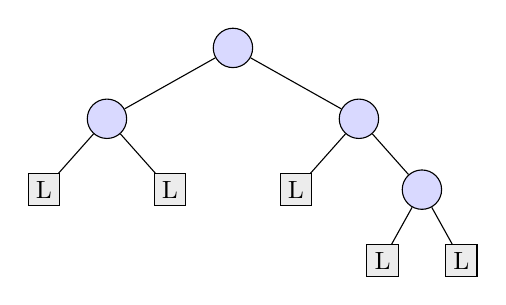
\begin{tikzpicture}[
    level distance=0.9cm,
    level 1/.style={sibling distance=3.2cm},
    level 2/.style={sibling distance=1.6cm},
    level 3/.style={sibling distance=1.0cm},
    every node/.style={font=\small},
    internal/.style={circle, draw, fill=blue!15, minimum size=5mm, inner sep=0pt},
    leaf/.style={rectangle, draw, fill=gray!15, minimum size=4mm, inner sep=1pt}
  ]
  \node[internal] {}
    child { node[internal] {}
      child { node[leaf] {L} }
      child { node[leaf] {L} }
    }
    child { node[internal] {}
      child { node[leaf] {L} }
      child { node[internal] {}
        child { node[leaf] {L} }
        child { node[leaf] {L} }
      }
    };
\end{tikzpicture}
\end{center}

Count by hand: there are 4 internal nodes (the blue circles) and 5 leaves (the gray squares), and you can trace 8 edges going down to children ($2 \times 4$, one pair per internal node). That's the pattern we're about to prove in general. The shapes $L$ stand for \texttt{Leaf} and the unmarked circles are \texttt{Node} constructors.

\subsection{Worked proof: counting edges in a binary tree}

Now let's prove something about binary trees using structural induction. We'll show that:

For all binary trees $t$:
\[
\texttt{edges}(t) = 2 \cdot \texttt{size}(t)
\]

In other words, a binary tree with $n$ internal nodes has exactly $2n$ edges (counting edges to leaf children). This makes intuitive sense: every node contributes exactly 2 edges (to its children), and leaves contribute 0.

We'll do structural induction on $t$. Our property $P(t)$ is the statement ``$\texttt{edges}(t) = 2 \cdot \texttt{size}(t)$.''

\textbf{Base case} ($t = \texttt{Leaf}$): We need $\texttt{edges(Leaf)} = 2 \cdot \texttt{size(Leaf)}$. The left side is $0$ and the right side is $2 \cdot 0 = 0$. Done.

\textbf{Inductive step} ($t = \texttt{Node(left, right)}$): Assume $P(\texttt{left})$ and $P(\texttt{right})$, i.e.\ assume:
\begin{align*}
\texttt{edges(left)} &= 2 \cdot \texttt{size(left)} && \text{(IH for left)} \\
\texttt{edges(right)} &= 2 \cdot \texttt{size(right)} && \text{(IH for right)}
\end{align*}

We need to show $\texttt{edges(Node(left, right))} = 2 \cdot \texttt{size(Node(left, right))}$.

Left side:
\begin{align*}
\texttt{edges(Node(left, right))} &= 2 + \texttt{edges(left)} + \texttt{edges(right)} && \text{(by definition of edges)} \\
&= 2 + 2 \cdot \texttt{size(left)} + 2 \cdot \texttt{size(right)} && \text{(by both IHs!)}
\end{align*}

Right side:
\begin{align*}
2 \cdot \texttt{size(Node(left, right))} &= 2 \cdot (1 + \texttt{size(left)} + \texttt{size(right)}) && \text{(by definition of size)} \\
&= 2 + 2 \cdot \texttt{size(left)} + 2 \cdot \texttt{size(right)}
\end{align*}

They're equal! Both sides give us $2 + 2 \cdot \texttt{size(left)} + 2 \cdot \texttt{size(right)}$, so $P(\texttt{Node(left, right)})$ holds. By structural induction, $P(t)$ for all binary trees $t$. $\square$

Notice how we used \textbf{both} inductive hypotheses in the inductive step---one for each subtree. That's the characteristic feature of tree induction: you get two IHs and you typically need both.

\section{The general recipe}

Let's spell out the pattern once and for all, because at this point you've seen it enough times that it should click.

Here's the recipe. Given \textbf{any} BNF definition of a datatype, you automatically get an induction principle. The correspondence is:

\begin{itemize}
  \item Each \textbf{base case} of the BNF gives you a \textbf{base case} of the proof. You need to show your property holds for each non-recursive constructor.
  \item Each \textbf{recursive case} of the BNF gives you an \textbf{inductive step}. For each recursive constructor, you get to \emph{assume} the property holds for all recursive sub-parts, and you need to \emph{show} it holds for the whole thing.
\end{itemize}

That's it. That's the whole recipe. Let's verify it against everything we've seen this quarter:

\textbf{Natural numbers:} $\texttt{Nat} := 0 \mid \texttt{succ Nat}$. One base case ($0$), one recursive case (\texttt{succ}) with one sub-part. So you get one base case and one inductive step with one IH. That's natural induction from Module 4.

\textbf{Lists:} $\texttt{List}\;A := \texttt{Nil} \mid \texttt{Cons}(A, \texttt{List}\;A)$. One base case (\texttt{Nil}), one recursive case (\texttt{Cons}) with one recursive sub-part (the tail). So you get one base case and one inductive step with one IH. Structurally identical to natural induction! And that makes sense: a list is basically a natural number that carries data.

\textbf{Binary trees:} $\texttt{BinTree} := \texttt{Leaf} \mid \texttt{Node}(\texttt{BinTree}, \texttt{BinTree})$. One base case (\texttt{Leaf}), one recursive case (\texttt{Node}) with \textbf{two} recursive sub-parts. So you get one base case and one inductive step with \textbf{two} IHs. That's the new thing we saw in this module.

And you could keep going! Imagine a datatype with two base cases and three recursive cases. You'd get two base cases and three inductive steps in your proof. Or consider propositional logic formulas from Module 2: $T$ and $F$ are base cases, ${\sim} L$ is a recursive case with one sub-part, and $L \wedge L$, $L \vee L$, $L \to L$ are recursive cases with two sub-parts each. So to prove something about all propositional formulas you'd handle the base cases ($T$, $F$, variables) and then do inductive steps for each connective, getting the appropriate number of inductive hypotheses each time.\footnote{If you go on to study programming languages or compilers, this is \emph{exactly} how you prove theorems about programs: by structural induction on the syntax of the language. The BNF of the programming language gives you the induction principle, and then you grind through the cases. It's this same recipe, just with bigger grammars.}

This extends to any datatype you can dream up---rose trees, abstract syntax trees, regular expressions, whatever. If you can write down a BNF for it, you get a structural induction principle for it. You'll see more of this in CS 251 when we work with graphs, automata, and other structures.

\subsection{Example: structural induction on propositional formulas}

Let's actually carry out that propositional-logic example instead of just waving at it. Recall the BNF from Module~2:

$L := T \mid F \mid x \mid {\sim} L \mid L \wedge L \mid L \vee L \mid L \to L$

Define a function \texttt{size} that counts the number of connectives in a formula:

\begin{lstlisting}
size(T)        = 0
size(F)        = 0
size(x)        = 0
size(~L)       = 1 + size(L)
size(L1 ^ L2)  = 1 + size(L1) + size(L2)
size(L1 v L2)  = 1 + size(L1) + size(L2)
size(L1 -> L2) = 1 + size(L1) + size(L2)
\end{lstlisting}

Seven cases, following the seven cases of the BNF---exactly the recipe we just described. Now let's prove a simple property to see the machinery work on a grammar with multiple base cases and multiple recursive cases.

\textbf{Claim.} For all formulas $f$, $\texttt{size}(f) \geq 0$.

We proceed by structural induction on $f$.

\textbf{Base cases.} If $f = T$, $f = F$, or $f = x$ (a variable), then $\texttt{size}(f) = 0 \geq 0$. Done.

\textbf{Inductive step (negation):} $f = {\sim} L$. Assume $\texttt{size}(L) \geq 0$ (IH). Then:
\begin{align*}
\texttt{size}({\sim} L) &= 1 + \texttt{size}(L) && \text{(by definition of \texttt{size})} \\
                        &\geq 1 + 0 = 1 \geq 0 && \text{(by IH)}
\end{align*}

\textbf{Inductive step (binary connectives):} $f = L_1 \star L_2$ where $\star$ is any of $\wedge$, $\vee$, $\to$. Assume $\texttt{size}(L_1) \geq 0$ (IH1) and $\texttt{size}(L_2) \geq 0$ (IH2). Then:
\begin{align*}
\texttt{size}(L_1 \star L_2) &= 1 + \texttt{size}(L_1) + \texttt{size}(L_2) && \text{(by definition of \texttt{size})} \\
                              &\geq 1 + 0 + 0 = 1 \geq 0 && \text{(by IH1 and IH2)}
\end{align*}

All cases handled. By structural induction, $\texttt{size}(f) \geq 0$ for every formula $f$. $\square$

The proof itself is almost trivially easy---and that's the point. What matters is the \emph{shape}: three base cases (matching the three non-recursive alternatives in the BNF), one inductive case with one IH (for ${\sim}$), and three inductive cases with two IHs each (for $\wedge$, $\vee$, $\to$). That shape was determined entirely by the BNF. We just followed the recipe.

\section{Wrapping up: the big picture}

Let's take a step back and look at what we've actually built over this whole course. There's been a single thread running through every module, and now we can finally state it cleanly.

The thread is a three-step pattern:
\begin{enumerate}
  \item \textbf{Define your data inductively} using BNF. Specify the base cases and the recursive cases.
  \item \textbf{Get an induction principle for free} that mirrors the structure of your definition. Base cases in the BNF become base cases in the proof. Recursive cases become inductive steps.
  \item \textbf{Use that principle to prove things} about all instances of your data by handling each case.
\end{enumerate}

We did this for propositional logic formulas in Module 2. We did this for natural numbers in Module 4. We did this for sequences in Module 8. In Module 9, we saw how \emph{strong} induction generalizes the basic induction principle to handle recurrences that reach back more than one step, and the characteristic equation technique gave us tools for solving those recurrences in closed form. And now in this module we've done it for lists and binary trees.

The specific data changes but the \emph{method} is always the same. Define inductively, get an induction principle, prove by cases. And as we saw in Module 8, this is the exact same thing as writing recursive programs: the structure of your data determines the structure of your code, which determines the structure of your proofs. Recursion, induction, and case analysis are facets of a single method depending on whether you're computing a value or proving a theorem.

If there's one thing I want you to take away from this course, it's this: when you encounter some new kind of structured data, the first question you should ask is ``what's the BNF?'' Once you have that, you know how to define functions on it (by recursion following the cases), and you know how to prove things about it (by induction following the cases). Everything else is details.

This is the foundation for CS 251 and beyond---type theory, programming language theory, algorithm analysis, formal verification. The datatypes get bigger and the proofs get harder, but the recipe stays the same. That recipe will carry you further than you might expect.\footnote{Okay, I lied a little. In CS 251 you'll see datatypes where the recursion is more complicated---mutual recursion, nested datatypes, indexed families---and the induction principles get correspondingly fancier. But the core idea really is the same. Promise.}

\section{Common mistakes}

\begin{enumerate}
  \item \textbf{Wrong number of inductive hypotheses.} The induction principle has exactly one IH per recursive sub-part in each recursive case. Students sometimes only use \emph{one} IH when proving a property of \texttt{Node(left, right)}---forgetting that they get \emph{both} $P(\texttt{left})$ and $P(\texttt{right})$. Conversely, students sometimes \emph{invent} IHs they don't have (e.g.\ claiming an IH for a parent tree when doing induction on a child). Always: IH count matches recursive-sub-part count in the BNF.
  \item \textbf{Missing a BNF case.} A structural induction proof has to handle every alternative in the BNF. If your grammar has seven alternatives (like the BNF for propositional formulas) and your proof handles five of them, you've proved a weaker statement than you think. For long grammars, explicitly list the cases at the top of the proof and check them off as you go.
  \item \textbf{Skipping the unfolding step.} The inductive step usually has the shape ``unfold the definition on the left, apply the IH, unfold the definition on the right, see they match.'' Students sometimes skip the unfolding and try to cite the IH directly on an expression where the IH doesn't actually apply---because the LHS expression has a $\texttt{Cons}$ or $\texttt{Node}$ wrapped around it and you have to \emph{unwrap} the definition first before the IH becomes applicable.
  \item \textbf{Generalizing the wrong variable.} When proving ``for all \texttt{xs} and \texttt{ys}, $\ldots$'', you usually induct on one of them with the \emph{other} universally quantified inside the predicate $P(\texttt{xs})$. If you fix a particular \texttt{ys} and then try to induct on \texttt{xs}, you might find your proof goes through---but you've only proved the result for that particular \texttt{ys}. To prove it for all \texttt{ys}, the quantifier has to be \emph{inside} $P$.
  \item \textbf{Proving a lemma you didn't state.} In the reverse-is-involution exercise (and others like it) you often need a side lemma---something like $\texttt{reverse}(xs \mathbin{++} ys) = \texttt{reverse}(ys) \mathbin{++} \texttt{reverse}(xs)$---before the main theorem can go through. Students sometimes use such a lemma mid-proof without proving it. If you need a lemma, prove it separately first (or note it and come back to it). Don't assume a useful-looking equation.
  \item \textbf{Forgetting that \texttt{Leaf} is a tree.} Base cases sometimes get short-changed because they seem trivial. But a ``trivial'' base case is still a required case; write it down explicitly and verify. The one-line base case is sometimes where the \emph{whole argument} hinges---for example, in the leaves-vs-size proof, $\texttt{leaves}(\texttt{Leaf}) = 1$ but $\texttt{size}(\texttt{Leaf}) = 0$, and you need that $0 + 1$ relationship to see why the inductive hypothesis delivers the right answer.
\end{enumerate}

\section{Summary and looking ahead}

\begin{keytakeaway}
  \item \emph{Structural induction}: every BNF definition gives you an induction principle, one case per BNF alternative, with one IH per recursive sub-part in each case.
  \item Natural induction is structural induction on $\text{Nat} := 0 \mid \text{succ Nat}$. List induction is structural induction on $\text{List} := \texttt{Nil} \mid \texttt{Cons}(A, \text{List})$. Tree induction gives you \emph{two} IHs (one per subtree). Propositional-formula induction gives you seven cases. Same recipe every time.
  \item The shape of your data determines the shape of your code (recursive functions), which determines the shape of your proofs (induction principles). Recursion, induction, and case analysis are three views of a single pattern.
  \item Serious structural induction proofs often involve \emph{lemma chains}: the main theorem depends on a helper lemma, which depends on a smaller helper, each proved by its own structural induction.
  \item Once you can name the shape of a data type, you can also name the ``right notion of sameness'' for values of that type by abstracting over some of the structure---lists up to reordering become multisets, binary trees up to relabeling become shapes, formulas up to logical equivalence become Boolean functions.
  \item That is the same move we already saw for sets (extensional equality, Module~1), formulas (logical equivalence, Module~2), and groups (isomorphism, Module~5). The intermezzo after Module~6 is the essay on the pattern.
\end{keytakeaway}

\begin{summarybox}
\textbf{What we built this module.} This is the capstone of the first term. The three-step pattern---(1) define your data inductively via BNF, (2) get an induction principle for free, (3) use it to prove things by case analysis---has been present from Module 2 (the BNF for propositional logic) through Module 4 (natural induction) to here. We've finally named it and seen it work on several concrete data types. This is the pattern that will carry you through CS 251 and beyond.

\medskip
\textbf{Looking ahead.} This is the end of the first-term notes. The intermezzi after this module (``The Algebra of Types,'' ``The Lambda Calculus'') round out the picture by showing that data types form a rich algebraic structure of their own and that there's a tiny universal programming language---$\lambda$-calculus---underneath everything we've been doing. In CS 251 you'll see mutual recursion, nested datatypes, indexed families, and eventually dependent types; the core recipe ``BNF gives you induction'' generalizes to all of it. And if you go further---into programming language theory, formal verification, or type theory---this module is the hinge on which the rest hangs.

If there's one thing to internalize from the whole first term, it's this: when you encounter some new kind of structured data, the first question to ask is ``what's the BNF?'' The answer tells you how to define functions on it and how to prove things about it. Everything else is details.
\end{summarybox}

\section{Exercises}

Organized into \textbf{warm-up} (mechanical practice with recursive definitions), \textbf{standard} (structural-induction proofs on lists and trees), \textbf{challenge} (deeper proofs, including the negation-free monotone result), and \textbf{connection} (programming and forward pointers). Solutions are in the appendix.

\subsection*{Warm-up}

\textbf{Exercise 1.}\label{ex:m10:1} Define a recursive function $\texttt{reverse}$ on lists, following the two cases of the BNF. (Hint: you will need to use \texttt{append} (\texttt{++}) in the recursive case.) Then compute $\texttt{reverse}(\texttt{Cons}(1, \texttt{Cons}(2, \texttt{Cons}(3, \texttt{Nil}))))$ step by step, showing each unfolding of the definition.

\bigskip
\textbf{Exercise 2.}\label{ex:m10:2} Compute the following by hand, unfolding the definitions step by step:
\begin{enumerate}[label=(\alph*)]
  \item $\texttt{length}(\texttt{Cons}(a, \texttt{Cons}(b, \texttt{Nil})))$
  \item $\texttt{Cons}(1, \texttt{Cons}(2, \texttt{Nil})) \mathbin{++} \texttt{Cons}(3, \texttt{Nil})$
  \item $\texttt{size}(\texttt{Node}(\texttt{Leaf}, \texttt{Node}(\texttt{Leaf}, \texttt{Leaf})))$
  \item $\texttt{edges}(\texttt{Node}(\texttt{Leaf}, \texttt{Node}(\texttt{Leaf}, \texttt{Leaf})))$
\end{enumerate}

\bigskip
\textbf{Exercise 3.}\label{ex:m10:3} For each of the following BNFs, state the shape of the structural induction principle: how many base cases and how many inductive steps, and how many IHs in each inductive step.
\begin{enumerate}[label=(\alph*)]
  \item $\texttt{Color} := \texttt{Red} \mid \texttt{Green} \mid \texttt{Blue}$
  \item $\texttt{RoseTree} := \texttt{Leaf}(A) \mid \texttt{Branch}(\texttt{List RoseTree})$ (hmm, this one is tricky because the recursive case contains a list of subtrees, not a fixed number---answer informally)
  \item $\texttt{Expr} := \texttt{Const}(\mathbb{Z}) \mid \texttt{Var}(\text{Name}) \mid \texttt{Add}(\texttt{Expr}, \texttt{Expr}) \mid \texttt{Mul}(\texttt{Expr}, \texttt{Expr}) \mid \texttt{Neg}(\texttt{Expr})$
\end{enumerate}

\subsection*{Standard}

\textbf{Exercise 4.}\label{ex:m10:4} Define a function $\texttt{leaves}(t)$ that counts the number of leaves in a binary tree (a \texttt{Leaf} counts as 1, a \texttt{Node} counts the leaves in both subtrees). Then prove by structural induction: $\texttt{leaves}(t) = \texttt{size}(t) + 1$ for all binary trees $t$. (You will need both inductive hypotheses in the inductive step, just like in the edges proof above.)

\bigskip
\textbf{Exercise 5.}\label{ex:m10:5} Define a function $\texttt{vars}(f)$ that returns the number of variable occurrences in a propositional formula (following the BNF from Module~2). For instance, $\texttt{vars}(x \wedge y) = 2$ and $\texttt{vars}(x \wedge x) = 2$ (we're counting occurrences, not distinct variables). Then prove by structural induction that for every formula $f$, $\texttt{vars}(f) \leq \texttt{size}(f) + 1$ (where $\texttt{size}$ is the connective-counting function defined in the module).

\bigskip
\textbf{Exercise 6.}\label{ex:m10:6} Prove by structural induction that append is associative on lists:
\[
  (xs \mathbin{++} ys) \mathbin{++} zs = xs \mathbin{++} (ys \mathbin{++} zs).
\]
Induct on $xs$, with $ys$ and $zs$ universally quantified inside the predicate.

\bigskip
\textbf{Exercise 7.}\label{ex:m10:7} Define $\texttt{map}(f, xs)$ recursively on lists: $\texttt{map}(f, \texttt{Nil}) = \texttt{Nil}$ and $\texttt{map}(f, \texttt{Cons}(x, xs')) = \texttt{Cons}(f(x), \texttt{map}(f, xs'))$. Prove by structural induction that $\texttt{length}(\texttt{map}(f, xs)) = \texttt{length}(xs)$ for every list $xs$.

\subsection*{Challenge}

\textbf{Exercise 8.}\label{ex:m10:8} Prove by structural induction that reverse is an involution:
\[
  \texttt{reverse}(\texttt{reverse}(xs)) = xs \quad \text{for every list } xs.
\]
You will need two helper lemmas:
\begin{enumerate}
  \item $xs \mathbin{++} \texttt{Nil} = xs$ for every $xs$. (Proof by induction on $xs$.)
  \item $\texttt{reverse}(xs \mathbin{++} ys) = \texttt{reverse}(ys) \mathbin{++} \texttt{reverse}(xs)$. (Proof by induction on $xs$, using the first lemma in the base case.)
\end{enumerate}
Prove both helpers, then use them to prove the main result. This is a good example of how real structural induction proofs often involve a chain of lemmas.

\bigskip
\textbf{Exercise 9.}\label{ex:m10:9} (The plan's request: a real semantic property.) Say a propositional formula is \emph{negation-free} if it is built from $T$, $F$, variables, and the connectives $\wedge$, $\vee$ only (i.e., the BNF excludes $\lnot$ and $\to$). Say a boolean function $f$ is \emph{monotone in variable $x$} if flipping $x$ from $F$ to $T$ (with all other variables held fixed) never flips the output of $f$ from $T$ to $F$. Prove by structural induction on the negation-free BNF:
\[
  \text{Every negation-free formula is monotone in every variable.}
\]
Hint: you'll need the sub-lemma that $\wedge$ and $\vee$ preserve monotonicity---if two functions are monotone in $x$, so is their conjunction and their disjunction. You can also look back at Module~2 Exercise~10, where you proved that $\{\wedge, \vee\}$ is not functionally complete using exactly this monotonicity idea.

\bigskip
\textbf{Exercise 10.}\label{ex:m10:10} A binary tree is \emph{perfect} if every non-leaf node has two subtrees of the same height. Define $\texttt{height}(t)$ recursively: $\texttt{height}(\texttt{Leaf}) = 0$ and $\texttt{height}(\texttt{Node}(l, r)) = 1 + \max(\texttt{height}(l), \texttt{height}(r))$. Prove by structural induction: for every perfect binary tree $t$, $\texttt{leaves}(t) = 2^{\texttt{height}(t)}$. (Hint: the definition of ``perfect'' is itself inductive: \texttt{Leaf} is perfect, and $\texttt{Node}(l, r)$ is perfect if $l$ and $r$ are both perfect and have the same height. Induct on the structure of the perfect tree.)

\subsection*{Connection}

\textbf{Exercise 11.}\label{ex:m10:11} (Programming.) Implement \texttt{List} and \texttt{BinTree} as Python classes following the BNFs. Then implement \texttt{length}, \texttt{append}, \texttt{reverse}, \texttt{size}, \texttt{edges}, \texttt{leaves}, \texttt{height} as methods or free functions. Write unit tests that check the theorems proved in the module and exercises: for instance, verify that $\texttt{length}(xs \mathbin{++} ys) = \texttt{length}(xs) + \texttt{length}(ys)$ holds on a handful of random lists. Use Python's \texttt{random} and maybe \texttt{hypothesis} (if you want a proper property-based testing library) to stress-test your implementations.

\bigskip
\textbf{Exercise 12.}\label{ex:m10:12} (Intermezzo pointer.) The ``Algebra of Types'' intermezzo that follows this module explains that BNF definitions correspond to \emph{polynomial functors}, and that the associated induction principles are cases of a general categorical theorem. As a warm-up, count the ``shape'' of each of the following datatypes by writing down a polynomial-like expression. For example, $\texttt{List}\,A := \texttt{Nil} \mid \texttt{Cons}(A, \texttt{List}\,A)$ corresponds to $L = 1 + A \cdot L$ (where $1$ stands for the \texttt{Nil} case with no data and $A \cdot L$ stands for \texttt{Cons} with an $A$ and a sub-list). Do the same for:
\begin{enumerate}[label=(\alph*)]
  \item $\texttt{Nat} := 0 \mid \texttt{succ Nat}$
  \item $\texttt{BinTree} := \texttt{Leaf} \mid \texttt{Node}(\texttt{BinTree}, \texttt{BinTree})$
  \item $\texttt{Maybe}\,A := \texttt{Nothing} \mid \texttt{Just}(A)$ (not recursive!)
\end{enumerate}
Why do you think the intermezzo calls these ``polynomial'' functors?

\end{document}
